% !TEX root = ../../../main.tex
% !TEX encoding = UTF-8 Unicode
% !TEX encoding = UTF-8

\clearpage

\subsection{Kostenarten in Hochschulen}
Im Hochschulbereich betrachtet man besonders die Kostenarten der Einzelkosten und Gemeinkosten. Die Kostenarten müssen, im universitären Umfeld, vorrangig in Forschungsprojekten mit Drittmitteln, genau aufgeschlüsselt und zugewiesen werden, um einen transparenten Überblick zu erhalten, wo die Kosten anfallen und wo die Drittmittel Verwendung finden.\footnote{\autocite[7]{pkl_2005}}

Die genaue Form der Kostenerfassung sollte in diesem Projekt angewendet werden. Es sollte eine sekundäre Kostenart Informationsmanagement geben, damit die Kosten zugeordnet und überwacht werden können. Daraus können folgende Projekte im Vorfeld besser eingeschätzt werden. Dies wird durch die Einzelkosten erreicht, wohingegen die Gemeinkosten in mehreren Bereichen der Hochschule anfallen und der Aufwand einer Einzelzuordnung nicht vertretbar oder zielführend ist.

Die kalkulatorischen Kosten teilen sich in die Zusatzkosten und Anderskosten. In der Abbildung \ref{fig_abgrenzung_aufwand}\footnote{\autocite[9-10]{pkl_2005}} sind diese Kosten tabellarisch eingeordnet. Anderskosten sind Kostenarten die noch nicht benannt sind oder erkannt werden, aber nicht in der laufenden Periode zugeordnet werden können. 

\begin{figure}[h!]
	\centering
	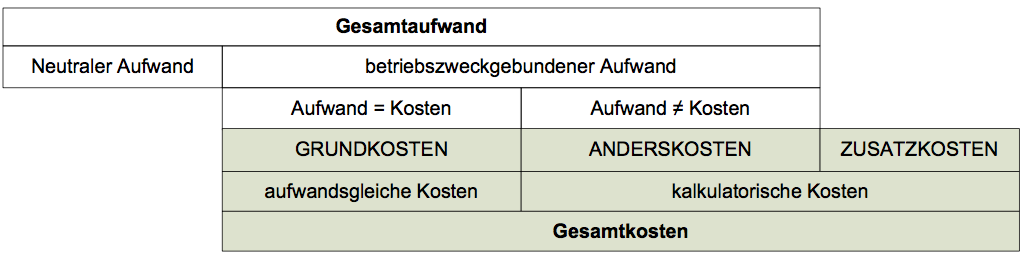
\includegraphics[width=\textwidth]
	{kapitel/gruppe4_2/bilder/abgrenzung_aufwand}
	\caption{Abgrenzung Aufwand-Kosten}
	\label{fig_abgrenzung_aufwand}
\end{figure}

In der Betrachtung der primären und sekundären Kostenarten, sind in einer Hochschule die sekundären Kostenarten besonders interessant, da sie die Kosten der Bereiche zusammenfassen und einen Überblick verschaffen.

Wie das Beispiel der Abbildung \ref{fig_uebergang_primaerkosten}\footnote{\autocite[10-11]{pkl_2005}} zeigt, bauen sich die sekundären Kosten, in der Kostenstellenrechung, durch das Zusammenfließen der primären Kosten auf. An der Leibnitz Universität Hannover (LUH) wurden, für das SAP-System, 900 Primärkostenarten in 140 Sekundärkostenarten verdichtet und zugeordnet.\footnote{\autocite[18]{pkl_2005}}

\begin{figure}[htp]
	\centering
	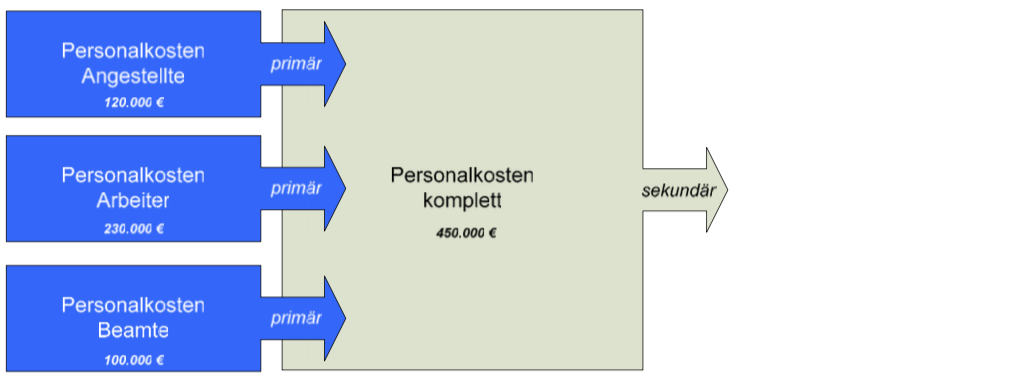
\includegraphics[width=0.75\textwidth]
	{kapitel/gruppe4_2/bilder/uebergang_primaerkosten}
	\caption{Übergang der Pimärkosten in Sekundärkosten}
	\label{fig_uebergang_primaerkosten}
\end{figure}

Diese Primärkostenarten und Sekundärkostenarten sind im Jahr 2005 im Rahmen des Projektes \enquote{Uni2001} für ganz Niedersachsen abgestimmt worden und im SAP-System eingepflegt.

\begin{figure}[h!]
	\centering
	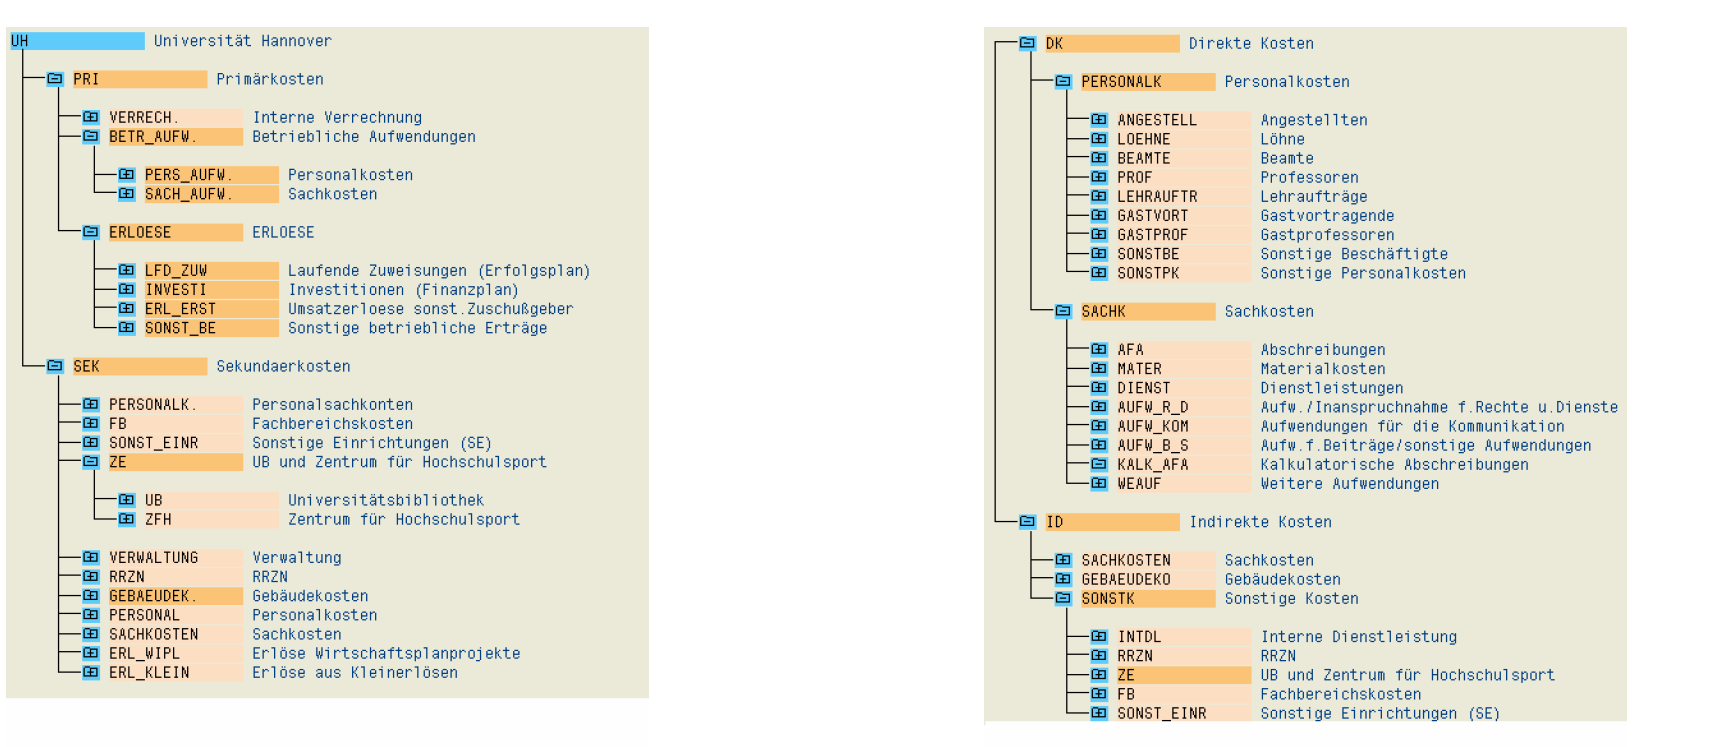
\includegraphics[width=\textwidth]
	{kapitel/gruppe4_2/bilder/kostenartenhierarchie_uni2001}
	\caption{Kostenartenhierarchie der Hochschulen Uni2001}
	\label{fig_kostenartenhierarchie_uni2001}
\end{figure}

Ein entsprechender Abgleich mit Mitarbeitern der Hochschule Emden/Leer für die vorhandenen und besonders der genutzten Kostenarten sollte bei der konkreten Projektplanung unbedingt erfolgen. Die Hierarchie der Kostenarten der Hochschule sollten sich ähnlich, wenn nicht sogar gleich, dem Beispiel der Abbildung \ref{fig_kostenartenhierarchie_uni2001}\footnote{\autocite[21]{pkl_2005}} der LUH darstellen.

\newpage